% Options for packages loaded elsewhere
% Options for packages loaded elsewhere
\PassOptionsToPackage{unicode}{hyperref}
\PassOptionsToPackage{hyphens}{url}
\PassOptionsToPackage{dvipsnames,svgnames,x11names}{xcolor}
%
\documentclass[
  10pt,
  letterpaper,
  DIV=11,
  numbers=noendperiod]{scrartcl}
\usepackage{xcolor}
\usepackage{amsmath,amssymb}
\setcounter{secnumdepth}{5}
\usepackage{iftex}
\ifPDFTeX
  \usepackage[T1]{fontenc}
  \usepackage[utf8]{inputenc}
  \usepackage{textcomp} % provide euro and other symbols
\else % if luatex or xetex
  \usepackage{unicode-math} % this also loads fontspec
  \defaultfontfeatures{Scale=MatchLowercase}
  \defaultfontfeatures[\rmfamily]{Ligatures=TeX,Scale=1}
\fi
\usepackage{lmodern}
\ifPDFTeX\else
  % xetex/luatex font selection
\fi
% Use upquote if available, for straight quotes in verbatim environments
\IfFileExists{upquote.sty}{\usepackage{upquote}}{}
\IfFileExists{microtype.sty}{% use microtype if available
  \usepackage[]{microtype}
  \UseMicrotypeSet[protrusion]{basicmath} % disable protrusion for tt fonts
}{}
% Make \paragraph and \subparagraph free-standing
\makeatletter
\ifx\paragraph\undefined\else
  \let\oldparagraph\paragraph
  \renewcommand{\paragraph}{
    \@ifstar
      \xxxParagraphStar
      \xxxParagraphNoStar
  }
  \newcommand{\xxxParagraphStar}[1]{\oldparagraph*{#1}\mbox{}}
  \newcommand{\xxxParagraphNoStar}[1]{\oldparagraph{#1}\mbox{}}
\fi
\ifx\subparagraph\undefined\else
  \let\oldsubparagraph\subparagraph
  \renewcommand{\subparagraph}{
    \@ifstar
      \xxxSubParagraphStar
      \xxxSubParagraphNoStar
  }
  \newcommand{\xxxSubParagraphStar}[1]{\oldsubparagraph*{#1}\mbox{}}
  \newcommand{\xxxSubParagraphNoStar}[1]{\oldsubparagraph{#1}\mbox{}}
\fi
\makeatother


\usepackage{longtable,booktabs,array}
\usepackage{calc} % for calculating minipage widths
% Correct order of tables after \paragraph or \subparagraph
\usepackage{etoolbox}
\makeatletter
\patchcmd\longtable{\par}{\if@noskipsec\mbox{}\fi\par}{}{}
\makeatother
% Allow footnotes in longtable head/foot
\IfFileExists{footnotehyper.sty}{\usepackage{footnotehyper}}{\usepackage{footnote}}
\makesavenoteenv{longtable}
\usepackage{graphicx}
\makeatletter
\newsavebox\pandoc@box
\newcommand*\pandocbounded[1]{% scales image to fit in text height/width
  \sbox\pandoc@box{#1}%
  \Gscale@div\@tempa{\textheight}{\dimexpr\ht\pandoc@box+\dp\pandoc@box\relax}%
  \Gscale@div\@tempb{\linewidth}{\wd\pandoc@box}%
  \ifdim\@tempb\p@<\@tempa\p@\let\@tempa\@tempb\fi% select the smaller of both
  \ifdim\@tempa\p@<\p@\scalebox{\@tempa}{\usebox\pandoc@box}%
  \else\usebox{\pandoc@box}%
  \fi%
}
% Set default figure placement to htbp
\def\fps@figure{htbp}
\makeatother





\setlength{\emergencystretch}{3em} % prevent overfull lines

\providecommand{\tightlist}{%
  \setlength{\itemsep}{0pt}\setlength{\parskip}{0pt}}



 


\usepackage{xcolor, soul}
\definecolor{Light}{gray}{.90}
\sethlcolor{Light}
\let\OldTexttt\texttt
\renewcommand{\texttt}[1]{\OldTexttt{\hl{#1}}}
\usepackage{caption}
\captionsetup{font=small, labelfont=bf}
\setlength{\parindent}{0pt}
\setlength{\parskip}{1.25ex}
\KOMAoption{captions}{tableheading}
\makeatletter
\@ifpackageloaded{caption}{}{\usepackage{caption}}
\AtBeginDocument{%
\ifdefined\contentsname
  \renewcommand*\contentsname{Table of contents}
\else
  \newcommand\contentsname{Table of contents}
\fi
\ifdefined\listfigurename
  \renewcommand*\listfigurename{List of Figures}
\else
  \newcommand\listfigurename{List of Figures}
\fi
\ifdefined\listtablename
  \renewcommand*\listtablename{List of Tables}
\else
  \newcommand\listtablename{List of Tables}
\fi
\ifdefined\figurename
  \renewcommand*\figurename{Figure}
\else
  \newcommand\figurename{Figure}
\fi
\ifdefined\tablename
  \renewcommand*\tablename{Table}
\else
  \newcommand\tablename{Table}
\fi
}
\@ifpackageloaded{float}{}{\usepackage{float}}
\floatstyle{ruled}
\@ifundefined{c@chapter}{\newfloat{codelisting}{h}{lop}}{\newfloat{codelisting}{h}{lop}[chapter]}
\floatname{codelisting}{Listing}
\newcommand*\listoflistings{\listof{codelisting}{List of Listings}}
\makeatother
\makeatletter
\makeatother
\makeatletter
\@ifpackageloaded{caption}{}{\usepackage{caption}}
\@ifpackageloaded{subcaption}{}{\usepackage{subcaption}}
\makeatother
\usepackage{bookmark}
\IfFileExists{xurl.sty}{\usepackage{xurl}}{} % add URL line breaks if available
\urlstyle{same}
\hypersetup{
  pdftitle={Randomized dichotomy d' calculations},
  pdfauthor={Al Xin},
  colorlinks=true,
  linkcolor={blue},
  filecolor={Maroon},
  citecolor={Blue},
  urlcolor={Blue},
  pdfcreator={LaTeX via pandoc}}


\title{Randomized dichotomy d' calculations}
\author{\small Al Xin}
\date{Jul 30, 2026}
\begin{document}
\maketitle


\section{Data}\label{data}

\subsection{Loading}\label{loading}

See \texttt{20260625.qmd} for reference. For now, analysis will be
limited to reliable sites and images with naturalistic structure.

\section{Methods}\label{methods}

\subsection{Mahalanobis distance}\label{mahalanobis-distance}

A multivariate distance value can be calculated with the typical
Mahalanobis distance formula, i.e., \[
d_M (\mathbf{x}, \mathbf{y}) = \sqrt{(\mathbf{x} - \mathbf{y})^\intercal \Sigma^{-1} (\mathbf{x} - \mathbf{y})},
\] where \(\mathbf{x}, \mathbf{y}\) correspond to the mean activity
vectors for each group, taken with respect to each site. The pooled
covariance matrix is the same as used in Hotelling's two-sample
statistic, derived as \[
\Sigma = 
\frac{(n_x - 1) \Sigma_x + (n_y - 1)\Sigma_y}{n_x + n_y - 2},
\] where \(\Sigma_x, \Sigma_y\) are the typical sample covariance
matrices for each distribution. \texttt{Rfast} contains functions
\texttt{Rfast::pooled.cov()} and \texttt{Rfast::spdinv()} to support
these calculations.

For low trial numbers, the inverse covariance matrix can be found with
the regularized/shrinkage estimator from
\texttt{corpcor::invcov.shrink()}. Though I did not find a meaningful
difference between the ordinary and shrinkage estimator for the
between-family comparison, there are fewer trials for the randomized
dichotomies and it may be worth performing the comparison again.

\subsection{Randomized dichotomies}\label{randomized-dichotomies}

Due to the low number of repetitions for each image (6 repetitions for
each unique image), it may be unstable to perform one-vs-one or
one-vs-all comparisons of specific sample instances. Instead, two groups
of 7 sample IDs each (without replacement) will be selected. Because
this is not an even split of the available sample IDs, the procedure
will proceed as follows:

\begin{enumerate}
\def\labelenumi{\arabic{enumi}.}
\tightlist
\item
  Omit one of the 15 IDs (1, 2, \ldots, 15)
\item
  Take a random sample of the possible \(\binom{14}{7}\) combos of the
  remaining indices.
\end{enumerate}

Given the above file of randomized dichotomies, the Mahalanobis distance
calculation proceeds similarly to \texttt{20260715.qmd}, with minor
modifications to how the groups are determined.

\section{Pairwise distances between
samples}\label{pairwise-distances-between-samples}

With only six samples, the inverse covariance matrix needs to be found
with a shrinkage estimator, such as the one provided by
\texttt{corpcor::invcov.shrink()}. When the distances are aggregated
over families, the pairwise distances tend to be largest for V2, a trend
that seems to be consistent when the values are separated by families
(Figure~\ref{fig-pairwise_dM}). This is somewhat inconsistent with
Ziemba et al.'s results, which found that samples were better separated
in V1.

\begin{figure}

\centering{

\pandocbounded{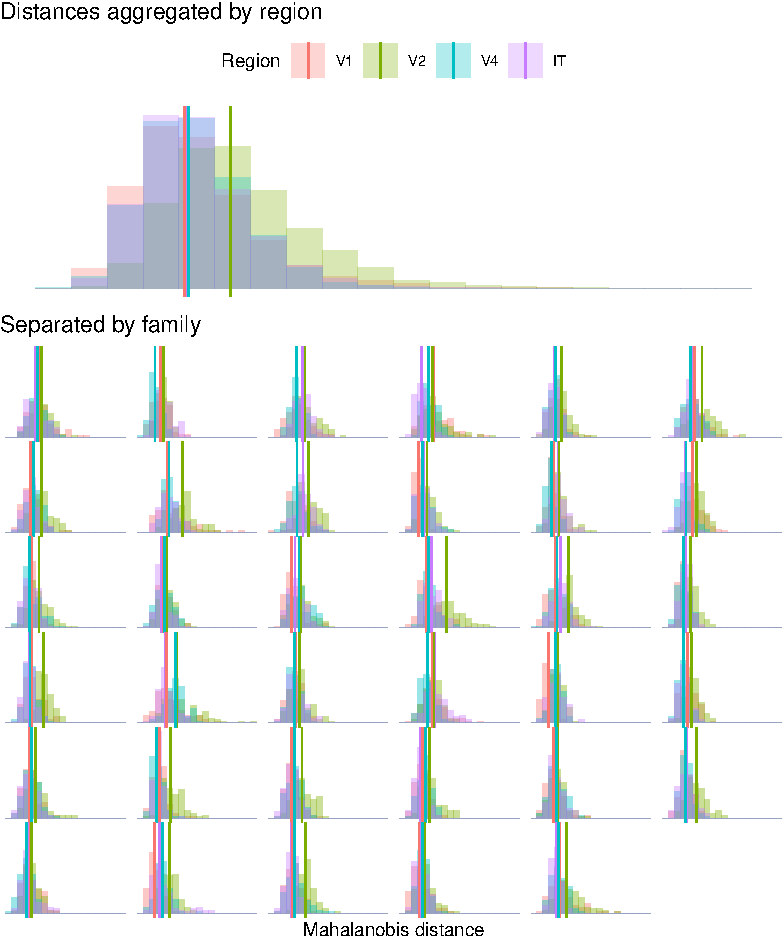
\includegraphics[keepaspectratio]{20260723_files/figure-pdf/fig-pairwise_dM-1.pdf}}

}

\caption{\label{fig-pairwise_dM}Histogram of Mahalanobis distances with
pairwise comparisons, separated by family and with fill color based on
region.}

\end{figure}%

\subsection{Randomized dichotomy
results}\label{randomized-dichotomy-results}

For convenience, since each of the randomized dichotomies needs to be
done within a family (of which there are 35), the initial results will
be saved in the Stats server.The initial results can be aggregated,
without further analysis of the within-family differences. I ran the
aggregation in the cluster and transferred the end result; see
\texttt{scripts/rd\_multi\_d\_agg.R}.

The randomized dichotomy results, in order of increasing median
distance, tends to follow V1 \textless{} IT \textless{} V4 \textless{}
V2, which is not consistent with the previous results in Ziemba et
al.~(2016). With the shrinkage estimator, the distribution of the
distances tends to be more concentrated around the median with less
extreme maximum distance values. Both the ordinary and shrinkage
estimators are right-skewed (Figure~\ref{fig-mahalanobis_shrinkage}).
The shrinkage estimator is probably more stable given the number of
repetitions. When assuming shrinkage, the number of sites used does not
change the overall pattern of the distances, but more sites tends to
increase the range of calculated distance values
(Figure~\ref{fig-mahalanobis_sites}). This does not change with the
ordinary (non-shrinkage) estimator (not shown).

\begin{figure}

\centering{

\pandocbounded{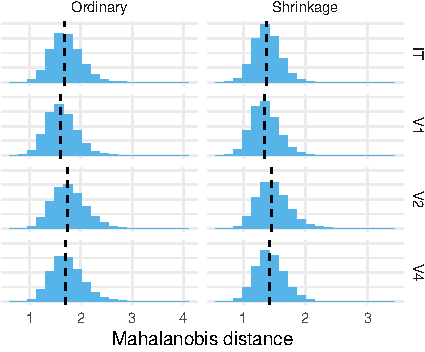
\includegraphics[keepaspectratio]{20260723_files/figure-pdf/fig-mahalanobis_shrinkage-1.pdf}}

}

\caption{\label{fig-mahalanobis_shrinkage}Histogram of Mahalanobis
distances with the ordinary covariance estimate (left) or the shrinkage
estimator (right) with samples of 30 sites.}

\end{figure}%

\begin{figure}

\centering{

\pandocbounded{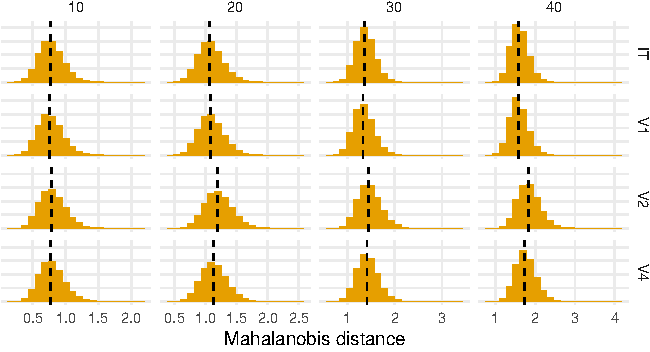
\includegraphics[keepaspectratio]{20260723_files/figure-pdf/fig-mahalanobis_sites-1.pdf}}

}

\caption{\label{fig-mahalanobis_sites}Histogram of Mahalanobis distances
with different numbers of sampled sites. Results are taken from the
shrinkage inverse covariance estimator.}

\end{figure}%




\end{document}
